\textbf{3.} \textbf{(2.5pts.)} Extender la siguiente gram\'atica con atributos para 
la regla $E \to E_1 * E_2$ y obtener el c\'odigo de tres direcciones para la 
expresi\'on $x = a[i][j] * b[i][j] $ donde $a$ y $b$ son arreglos de tama\~no
$2\times 3$ y $2\times 2$ respectivamente y cada uno de ellos almacena enteros 
cuyo tama\~no es $4$.
\begin{center}
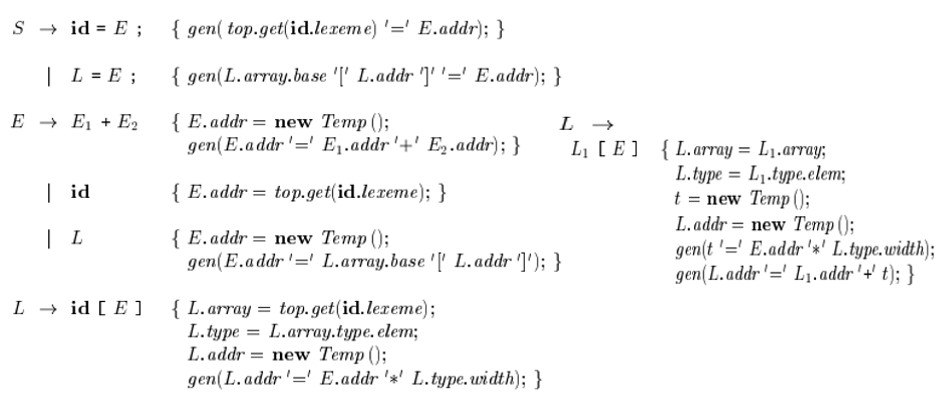
\includegraphics[width=.85\textwidth]{./ArrayRef}
\end{center}

\begin{table}[h]
    \centering
    \caption{Gramatica Extendida}
    \label{tab:Gramatica Extendida}
    \begin{tabular}{l l l}

         & & \\
        $S$ & $\rightarrow id = E;$ & $\{gen(top.get(id.lexeme) '=' E.addr);\}$\\
         & & \\
         & $|L = E;$ & $\{gen(L.array.base'['L.addr']' '=' E.addr);\}$ \\
         & & \\
        $E$ & $\rightarrow E_1 + E_2$ & $\{E.addr = new$ $Temp (); $\\
         & & $gen(E.addr '=' E_1.addr '+' E_2.addr); \}$ \\
         & & \\
         & $| E_1 * E_2$ & $\{E.addr = new$ $Temp (); $\\
         & & $gen(E.addr '=' E_1.addr '*' E_2.addr); \}$ \\
         & & \\
         & $| id$ & $\{E.addr = top.get(id.lexeme); \}$ \\
         & & \\
         & $| L$ & $\{E.addr = new$ $Temp();$\\
         & & $ gen(E.addr'='L.array.base'['L.addr']'); \}$ \\
         & & \\
        $L$ & $\rightarrow id [ E ]$ & $\{L.array = top.get(id.lexeme);$\\
         & & $$ $L.type = L.array.type.elem;$\\
         & & $ L.addr = new$ $Temp();$\\
         & & $$ $gen(L.addr '=' E-addr '*' L.type.width); \}$ \\
         & & \\
         & $| L_1 [ E ]$ & $\{L.array = L_1.array;$\\
         & & $ L.type = L_1.array.type.elem;$\\
         & & $ t = new$ $Temp();$\\
         & & $ gen(t '=' E.addr '*' L.type.width);$\\
         & & $ gen(L.addr '= L_1.addr '+' t); \}$ \\

    \end{tabular}
    
\end{table}

\begin{figure}[h!]
    \centering
    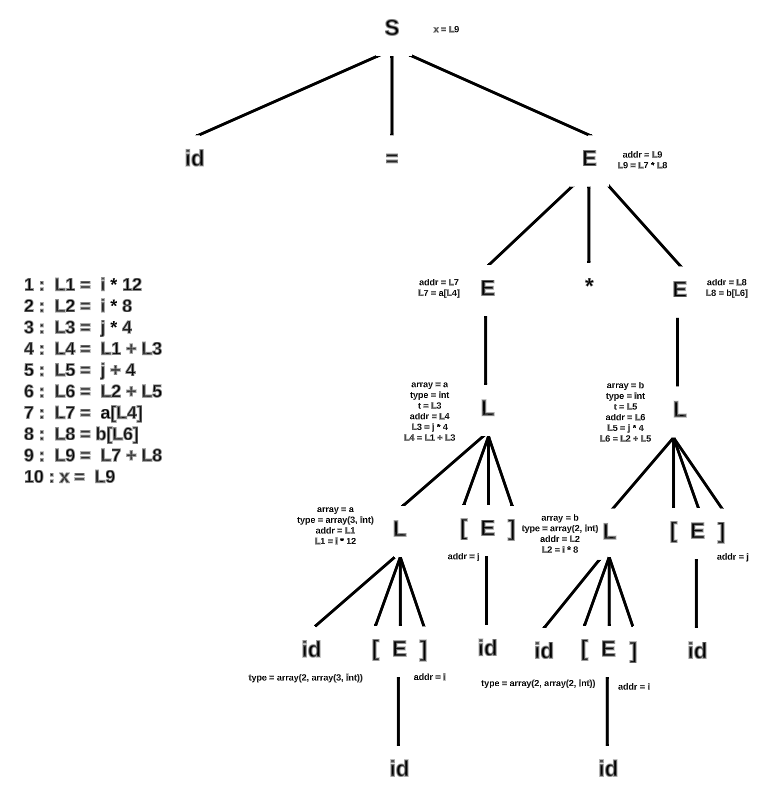
\includegraphics[scale = 0.75]{3_tres_direcciones}
    \caption{Codigo tres direcciones}
    \label{fig:Codigo tres direcciones}
\end{figure}

